% XeLaTeX

\documentclass{article}
\usepackage{ctex}
\usepackage{xypic}
\usepackage{amsfonts,amssymb}
\usepackage{multirow}
\usepackage{geometry}
\usepackage{graphicx}
\usepackage{listings}
\usepackage{lipsum}
\usepackage{courier}
\usepackage{fancyvrb}
\usepackage{etoolbox}


\linespread{1.2}
\geometry{left=3cm,right=2.5cm,top=2.5cm,bottom=2.5cm}

\makeatletter
\patchcmd{\FV@SetupFont}
  {\FV@BaseLineStretch}
  {\fontencoding{T1}\FV@BaseLineStretch}
  {}{}
\makeatother

\lstset{basicstyle=\small\fontencoding{T1}\ttfamily,breaklines=true}
\lstset{numbers=left,frame=shadowbox,tabsize=4}
%\lstset{extendedchars=false}
\begin{document}

\title{实验七 \text{ } 译码显示电路 \text{ } 实验报告}
\author {16337233 王凯祺}
\maketitle

\section{实验目的}

1. 掌握中规模集成译码器的逻辑功能和使用方法

2. 熟悉数码管的使用

\section{实验仪器}

1. 数字电路实验箱、数字万用表、示波器

2. 器件: 74LS48、74LS194、74LS73、74LS00

\section{实验内容}

\subsection{测试 74LS194}

将 $D_0$ 接低电平 ,$D_1, D_2, D_3, \overline{Cr}$ 接高电平,将 $S_0, S_1, D_{SL}, D_{SR}$ 接拨码开关, $CP$ 接单步脉冲, $Q_0, Q_1, Q_2, Q_3$ 接 01 显示器,观察输出结果。

\subsection{测试四节拍顺序发生器}

CP 脉冲上升沿和下降沿的输入顺序都可以实现四节拍顺序发生器。

CP 脉冲上升沿先到来时, 74LS194 先工作,74LS73 后工作。当 $Q_3$ 为 0 时,$J = K = 1$ ,故在下降沿到来时将 Q 取反,使得 $\overline{Q} = 1$ ,在下一时刻上升沿到来时实现并行送数。当 $Q_3$ 为 1 时,$J = 1, K = 0$ ,故在下降沿到来时将 $\overline{Q}$ 置为 0 ,实现右移。

CP 脉冲下降沿先到来时, 74LS73 先工作,74LS194 后工作。初始时 $Q_3$ 为 0 ,故 $K = 1$ ,$\overline{Q} = 1$ ,实现并行送数,之后与 CP 脉冲上升沿先到来的工作原理无异。

\subsection{四位扫描译码显示电路}

采用顺序脉冲作为 Ds 信号,8421 BCD 码用逻辑模拟开关输入,观察七段数码管的输出。

\newpage

\subsection{在 LED 数码管上同时显示出 8 位学号}

\subsubsection{显示内容决定显示位置}

这个比较简单。用 74LS197 产生八进制计数,接入数码管段选端,将显示内容的 BCD 码作为地址码接入 74LS138 地址输入端,将 74LS138 的输出连接到数码管对应位的位选端即可。

\subsubsection*{Proteus 电路设计}

\begin{figure}[!hbp]
  \centering
  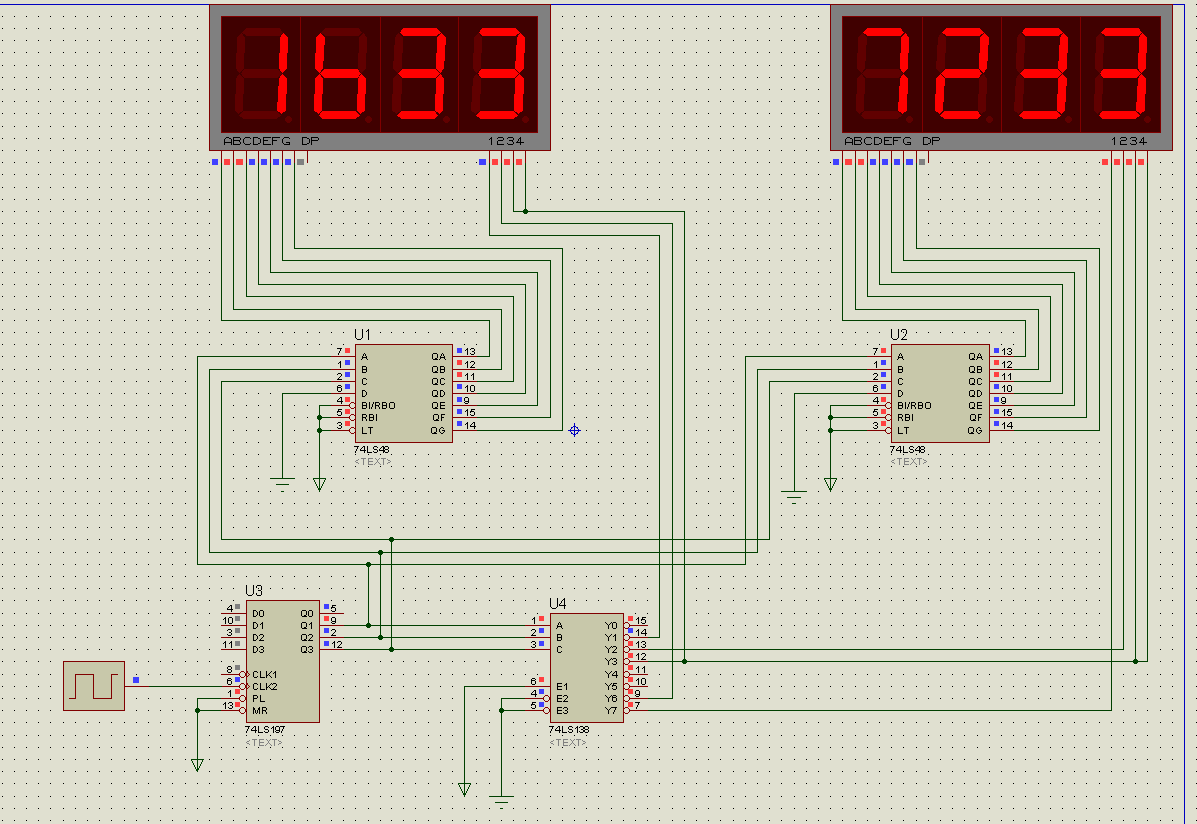
\includegraphics[scale=0.3]{lab7-1.png}
\end{figure}

\newpage

\subsubsection*{实验箱实现}

\begin{figure}[!hbp]
  \centering
  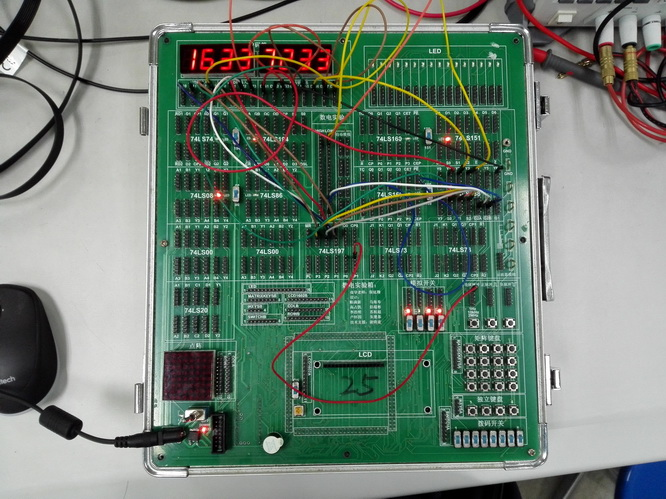
\includegraphics[scale=0.5]{IMG_20170503_083820.jpg}
\end{figure}

\begin{figure}[!hbp]
  \centering
  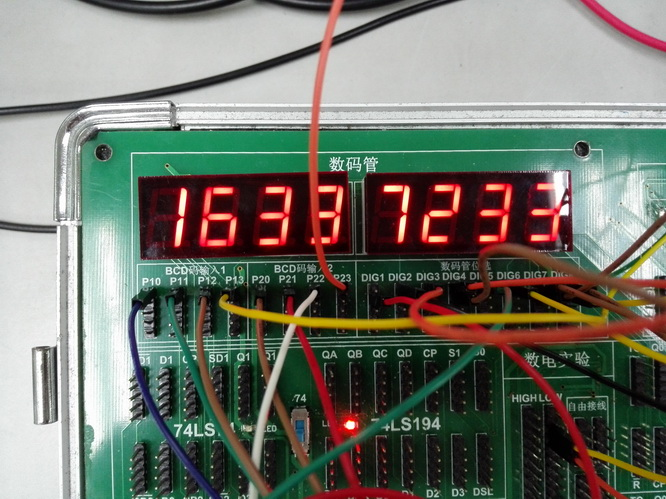
\includegraphics[scale=0.5]{IMG_20170503_083821.jpg}
\end{figure}

\newpage

\subsubsection{显示位置决定显示内容}

通过 74LS194 作为四节拍顺序脉冲发生器,输出分别连入两块 4 位数码管的位选端,控制数码管从第 1 位到第 4 位扫描的同时从第 5 位到第 8 位扫描。确定了显示位置后,通过画卡诺图的方法,输入是位选端,输出是段选端,设计出组合逻辑电路。

由于前 4 位的设计与后 4 位的设计是一样的,这里只写后 4 位的设计。

真值表:

\begin{table}[!hbp]
\centering
\begin{tabular}{|c|c|c|c||c|c|c|c|}
\hline
dig1 & dig2 & dig3 & dig4 & p3 & p2 & p1 & p0 \\
\hline
0 & 1 & 1 & 1 & 0 & 1 & 1 & 1 \\
\hline
1 & 0 & 1 & 1 & 0 & 0 & 1 & 0 \\
\hline
1 & 1 & 0 & 1 & 0 & 0 & 1 & 1 \\
\hline
1 & 1 & 1 & 0 & 0 & 0 & 1 & 1 \\
\hline

\end{tabular}

\end{table}

容易得到:

$p3 = 0$

$p2 = \overline{dig1}$

$p1 = 1$

$p0 = dig2$


\subsubsection*{Proteus 电路设计}

\begin{figure}[!hbp]
  \centering
  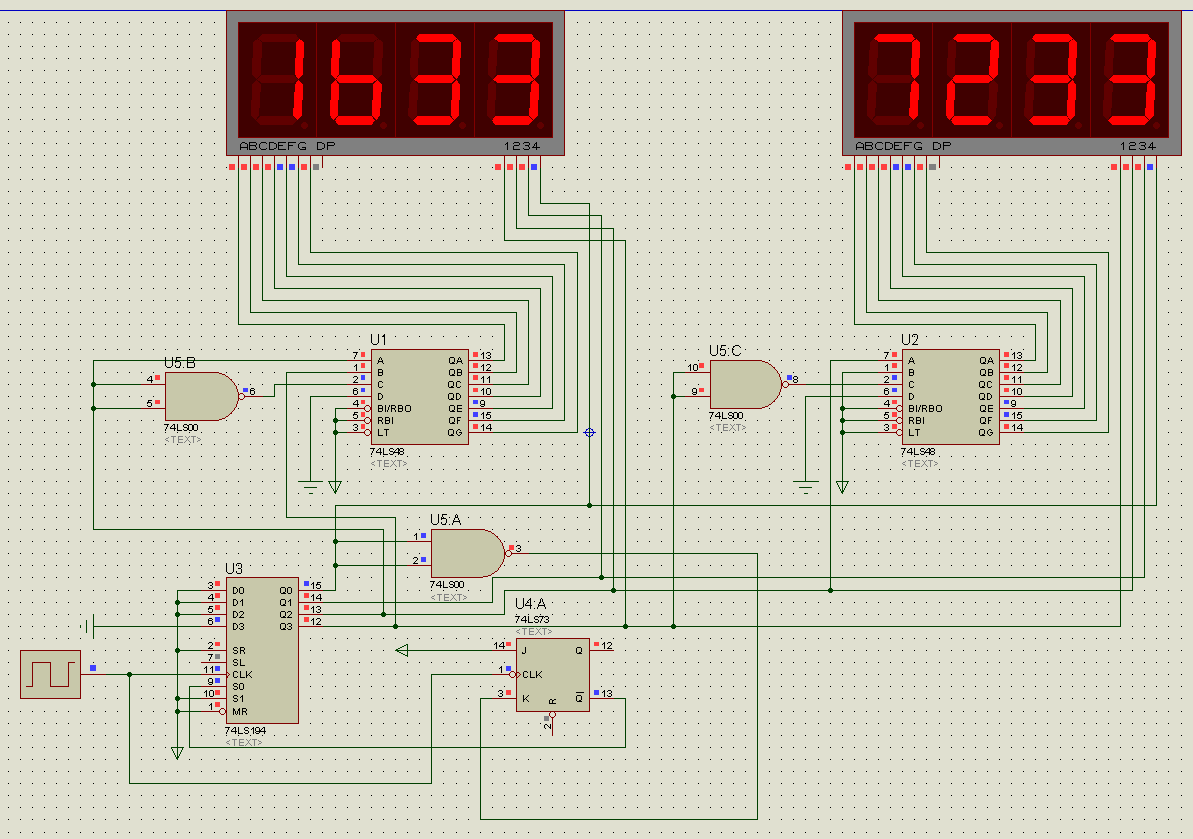
\includegraphics[scale=0.3]{lab7-2.png}
\end{figure}

\newpage

\subsubsection*{实验箱实现}

\begin{figure}[!hbp]
  \centering
  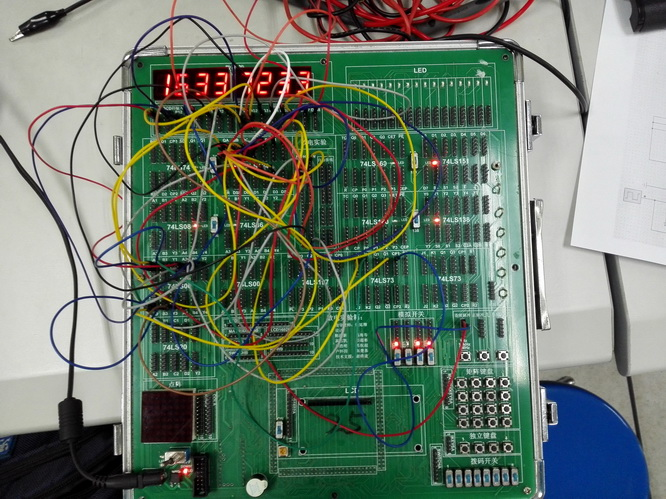
\includegraphics[scale=0.5]{IMG_20170503_083818.jpg}
\end{figure}

\begin{figure}[!hbp]
  \centering
  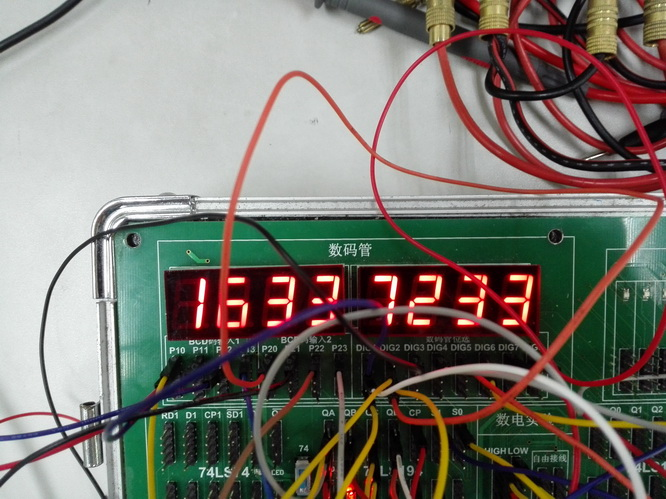
\includegraphics[scale=0.5]{IMG_20170503_083819.jpg}
\end{figure}

\end{document}
















